\documentclass[a4paper,14pt]{extreport}
  \usepackage[left=1.5cm,right=1.5cm,
      top=1.5cm,bottom=2cm,bindingoffset=0cm]{geometry}
  \usepackage{scrextend}
  \usepackage[T1,T2A]{fontenc}
  \usepackage[utf8]{inputenc}
  \usepackage[english,russian,ukrainian]{babel}
  \usepackage{tabularx}
  \usepackage{amssymb}
  \usepackage{color}
  \usepackage{amsmath}
  \usepackage{mathrsfs}
  \usepackage{listings}
  \usepackage{graphicx}
  \graphicspath{ {./images/} }
  \usepackage{lipsum}
  \usepackage{xcolor}
  \usepackage{hyperref}
  \usepackage{tcolorbox}
  \usepackage{tikz}
  \usepackage[framemethod=TikZ]{mdframed}
  \usepackage{wrapfig,boxedminipage,lipsum}
  \mdfdefinestyle{MyFrame}{%
  linecolor=blue,outerlinewidth=2pt,roundcorner=20pt,innertopmargin=\baselineskip,innerbottommargin=\baselineskip,innerrightmargin=20pt,innerleftmargin=20pt,backgroundcolor=gray!50!white}
   \usepackage{csvsimple}
   \usepackage{supertabular}
  \usepackage{pdflscape}
  \usepackage{fancyvrb}
  %\usepackage{comment}
  \definecolor{ggreen}{rgb}{0.4,1,0}
  \definecolor{rred}{rgb}{1,0.1,0.1}
  \usepackage{array,tabularx}
  \usepackage{colortbl}

  \usepackage{varwidth}
  \tcbuselibrary{skins}
  \usepackage{fancybox}

  \definecolor{ggreen}{rgb}{0.4,1,0}
  \definecolor{rred}{rgb}{1,0.1,0.1}
  \definecolor{amber}{rgb}{1.0, 0.75, 0.0}
  \definecolor{babyblue}{rgb}{0.54, 0.81, 0.94}
  \definecolor{asparagus}{rgb}{0.53, 0.66, 0.42}
  \definecolor{chartreuse}{rgb}{0.5, 1.0, 0.0}
  \definecolor{darkorchid}{rgb}{0.6, 0.2, 0.8}
  \usepackage{fp}

  \usepackage{float}
  \usepackage{wrapfig}
  \usepackage{framed}
  %for nice Code{
  \lstdefinestyle{customc}{
    belowcaptionskip=1\baselineskip,
    breaklines=true,
    frame=L,
    xleftmargin=\parindent,
    language=C,
    showstringspaces=false,
    basicstyle=\small\ttfamily,
    keywordstyle=\bfseries\color{green!40!black},
    commentstyle=\itshape\color{purple!40!black},
    identifierstyle=\color{blue},
    stringstyle=\color{orange},
  }
  \lstset{escapechar=@,style=customc}
%}


\begin{document}

\newtcbox{\xmybox}[1][red]{on line, arc=7pt,colback=#1!10!white,colframe=#1!50!black, before upper={\rule[3pt] {0pt}{10pt}},boxrule=1pt,boxsep=0pt,left=6pt,right=6pt,top=2pt,bottom=2pt}


\pagecolor{white}
\begin{titlepage}
  \begin{center}
  \large
  Національний технічний університет України \\ "Київський політехнічний інститут імені Ігоря Сікорського"


  Факультет Електроніки

  Кафедра мікроелектроніки
  \vfill

  \textsc{ЗВІТ}\\

  {\Large Про виконання ІКР №4\\
  з дисципліни: «Твердотільна електроніка-2»\\[1cm]

  Пасивні елементи напівпровідникових
  ІМС. Дифузійні резистори.

  }
  \bigskip
  \end{center}
  \vfill

  \newlength{\ML}
  \settowidth{\ML}{«\underline{\hspace{0.4cm}}» \underline{\hspace{2cm}}}
  \hfill
  \begin{minipage}{1\textwidth}
  Виконавець:\\
  Студент 3-го курсу \hspace{4cm} $\underset{\text{(підпис)}}{\underline{\hspace{0.2\textwidth}}}$  \hspace{1cm}А.\,С.~Мнацаканов\\
  \vspace{1cm}

  Перевірив: \hspace{6.1cm} $\underset{\text{(підпис)}}{\underline{\hspace{0.2\textwidth}}}$  \hspace{1cm}О.\,В.~Мачулянський\\

  \end{minipage}

  \vfill

  \begin{center}
  2021
  \end{center}
\end{titlepage}


\begin{center}ЗАВДАННЯ\end{center}
\renewcommand{\labelenumii}{\arabic{enumi}.\arabic{enumii}.}
\begin{enumerate}
  \item Ознайомитись з методикою розрахунку інтегральних конденсаторів на основі p-n-переходів.
  \item Реалізувати інтегральний конденсатор на основі p-n-переходу (планарно-епітаксіальна технологія) з заданими
  параметрами: номінальна ємність С ; робоча напруга Uр; пробивна напруга Uпроб; добротність Q; глибина залягання p-n-переходу - хj.
  \begin{enumerate} 
    \item  Провести аналіз вихідних даних наведених в таблиці та вибрати тип інтегрального дифузійного конденсатора (ДК) (p-n-перехід на основі якого формується ДК).
    \item  Визначити геометричні розміри ДР.
    \item Оцінити внесок в загальну ємність ДК бічної частини p-n-переходу.
  \end{enumerate}
\end{enumerate}

\vspace{2 cm}

\begin{table}[h]
  \begin{center}
    \begin{tabular}{|c|c|c|c|c|c|c|}
    \hline
    Варіант & С, пФ & $\delta$ C, \% & $U_p$, B & $U_{\text{проб}}$, B & Q  & $x_j$, мкм \\ \hline
    5       & 20    & 20             & 10       & 70                   & 10 & 4          \\ \hline
    \end{tabular}
  \end{center}
\end{table}

Виходячи з вихідних даних маю p-n-перехід база-колектор.

\begin{figure}[h!]
\center{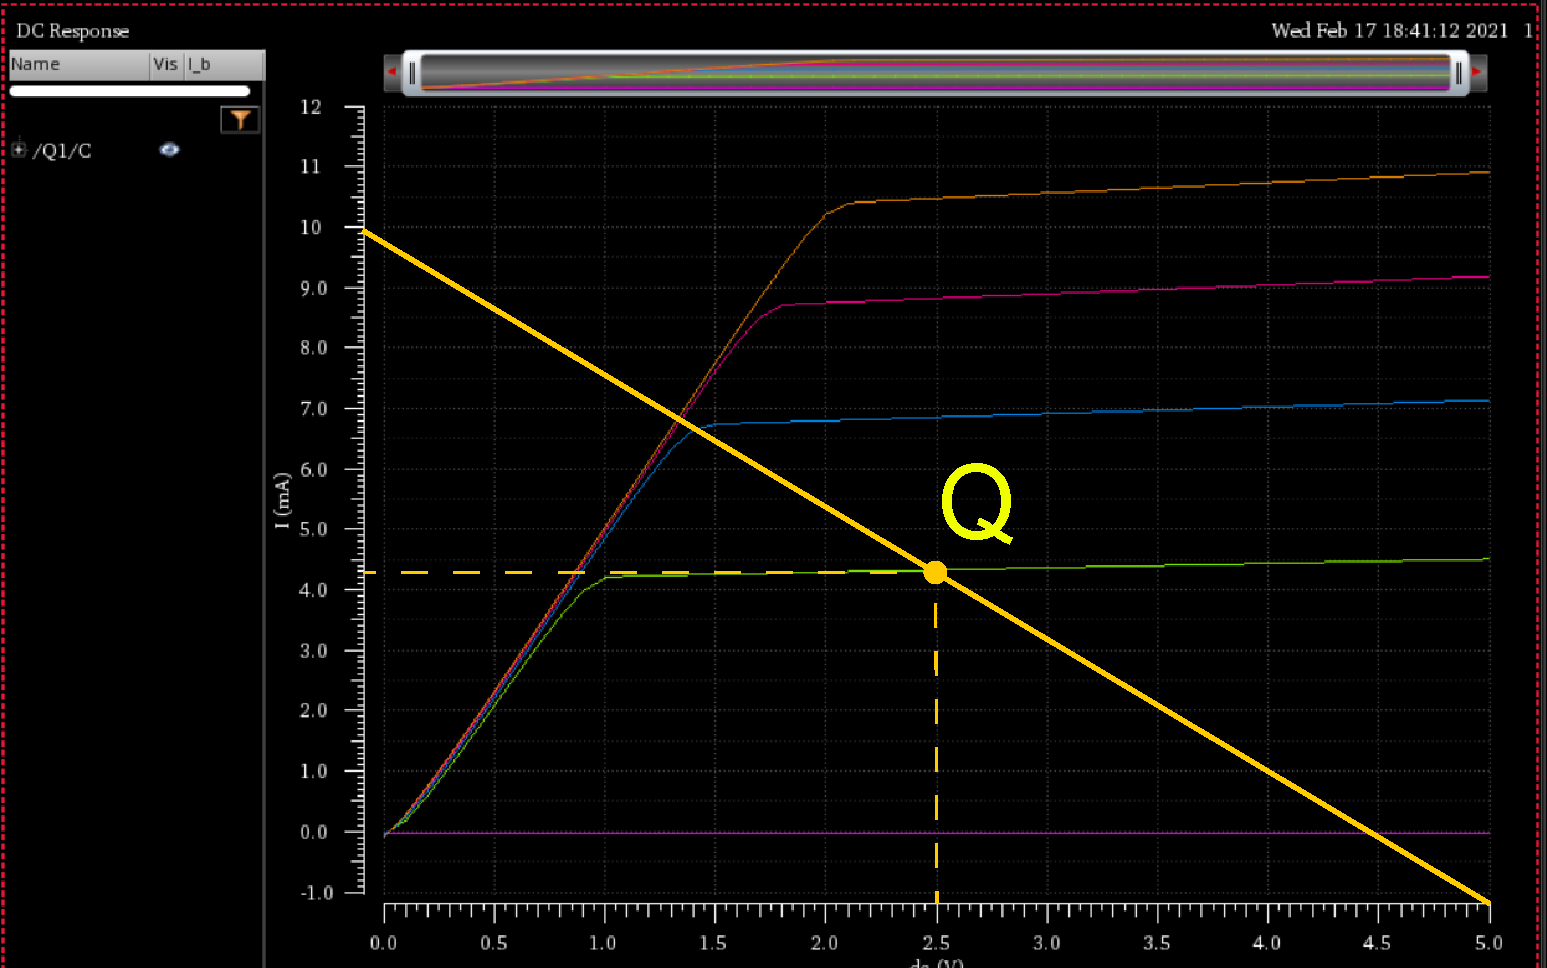
\includegraphics[width=0.7\linewidth]{1.png}}
\caption{Повна поверхня p-n-переходу}
\end{figure}
Ємнiсть дифузiйного конденсатора визначається за формулою:
\begin{align}
C = C_{\text{дон}} + C_{\text{бок}} = C_0\cdot S_{\text{дон}} + C_{0b}\cdot S_{\text{біч}},
\end{align}

де $S_{\text{дон}} = a\cdot b$, $S_{\text{цил}} = 2\cdot \pi \cdot \pi \cdot h$, $_{\text{сф}} = 4\cdot \pi \cdot r^2$ $r = x_j = 4 \text{ мкм}, h = a$\\

Беремо вiдношення сторiн a/b= 1, оскiльке воно забезпечить мiнiмальну
бокову ємнiсть.
$$
C=C_{0} \cdot a^{2}+C_{06} \times\left(\frac{4}{4} \cdot 2 \cdot \pi \cdot x_{j} \cdot a+\frac{4}{8} \cdot 4 \cdot \pi \cdot x_{j}^{2}\right)
$$
\begin{center}
$\Downarrow$
a = 0,337
\end{center}
$$C_{\text{дон}} = C_0 \cdot a^2 = 150 \cdot 10^{-12} \cdot 0,337= 17 \cdot 10^{-12}$$

$$
C_{\text {бок }}=C_{06} \times\left(\frac{4}{4} \cdot 2 \cdot \pi \cdot x_{j} \cdot a+\frac{4}{8} \cdot 4 \cdot \pi \cdot x_{j}^{2}\right)=2,99 \cdot 10^{-12} \Phi
$$

Склавши цi два значення ємностi отримаємо 20 пФ, що збiгається з теоретичними даними, i ємнiсть бiчної частини p-n переходу майже не впливає, а на загальну ємнiсть впливає донна ємнiсть.


%\FPeval\lrozp{round(\bprom* (\R/\ros - 2*\n*\kk - 0.55*\Nb):7 )}
%$$ L_{\text{розп}} = \bprom \cdot \left( \dfrac{\R}{\ros} - \n \kk - \n \kk - 0,55\cdot \Nb \right) = \lrozp  = 401 \text{ мкм}$$ 



%\FPeval\aaa{\P*\L*\bprom} 
%\aaa







%\begin{center}\fbox{\fcolorbox{black}{amber}{1}}\end{center}




%\clearpage
%\begin{center}\fbox{\fcolorbox{black}{babyblue}{2}}\end{center}




























\end{document}
